\chapter{\Zee\ cross section measurement}
\label{sec:ZeeCrossSec}

The measurement of the \Zee\ decay process is the main purpose of this work, and in this chapters the details of the methodology of this measurement would be discussed. The differential cross-sections are calculated using the Bayesian iterative unfolding with 3 iterations. The Bayesian unfolding is in some sense an evolution of the more primitive bin-by-bin unfolding, but the idea behind it is the same. But we will describe the unfolding methodology based on bin-by-bin, since it is more direct and is easier to explain.

The formulae for both integrated and differential cross-sections are:
\begin{equation}
\sigma_{tot} = \sigma_{Z} \times BR(\Zee) = \frac{N - B}{C \cdot E \cdot A \cdot L_{int}  \cdot \Gamma}\,,
\end{equation}
where:
\begin{itemize}
\item {\bfseries $N$} is the number of candidate events measured in data.
\item {\bfseries $B$} is the number of background events (see Sec.~\ref{sec:Bkg} for further information on the background estimation).
\item {\bfseries $L_{int}$} is the integrated luminosity corresponding to the run.
\item {\bfseries $\Gamma$} is the bin width for differential measurements. Measurements in rapidity quantities $\eta$ and $y$ are done in absolute binning as final value, i.e. $N$ is summed over positive and negative bin and $\Gamma$ is doubled.
\item $C$, $E$, and $A$ are efficiency-acceptance corrections calculated from (binned) sum of weights of MC events generated or reconstructed with various cuts applied. They take the uncorrected event yield in steps to different levels:
  \begin{itemize}
  \item The \textit{genuinely experimental fiducial volume in each channel} as defined by the individual cuts is reached after dividing by
    \begin{equation}
      C = \frac{N_\mathrm{MC, rec}}{N_\mathrm{MC, gen, cutexp}}\,.
    \end{equation}
    $C$ is corrected for any discrepancy in the electron efficiencies between data and MC as described in Sec.~\ref{sec:Efficiency}. Here the sum of weights of MC events generated after experimental fiducial acceptance cuts ($N_\mathrm{MC, gen, cutexp}$) and the sum of weights of MC events after simulation, reconstruction and experimental selection ($N_\mathrm{MC, rec}$) enter.
  \item The \textit{common fiducial volume} is a small theoretical extrapolation designed to unify the fiducial volumes of different flavors of \Zll\ analyses. Since the electrons and muons are detected by the different parts of the ATLAS detector, these particles are detected in different parts of the kinematic space. The EM calorimeters that detect electrons have a coverage of $|\eta| < 5.2$, while muon chambers have $|\eta| < 2.4$. These differences in the kinematic coverage makes combining the results of the corresponding analyses a challenge, which resulted in intruduction of the common fiducial volume which covers both kinematic spaces.
    \begin{equation}
      E = \frac{N_\mathrm{MC, gen, cutexp}}{N_\mathrm{MC, gen, cutfid}}\,.
    \end{equation}
    Here the sum of weights of MC events generated after common fiducial acceptance cuts ($N_\mathrm{MC, gen, cutfid}$) enters.
  \item \textit{Total cross sections} are reached by a larger theoretical extrapolation
    \begin{equation}
      A = \frac{N_\mathrm{MC, gen, cutfid}}{N_\mathrm{MC, gen, all}}\,.
    \end{equation}
    Here the total sum of weights of MC events generated before any acceptance cuts except $m_{ee}$ ($N_\mathrm{MC, gen, all}$) enters.
  \end{itemize}
\end{itemize}

The main difference in the results of the Bayesian and bin-by-bin unfoldings lies in two important factors: purity and stability. These two factors are calculated as follows:
\begin{equation}
P^{i} = \frac{N^{i}_{\text{rec\&gen}} }{ N^{i}_{\text{rec}} }\,, \; \;
S^{i} = \frac{N^{i}_{\text{rec\&gen}} }{ N^{i}_{\text{gen}} }\,,
\end{equation}
where:
\begin{itemize}
\item {\bfseries $N^i_{\text{rec\&gen}}$} is the sum of event weights which were generated and reconstructed in bin $i$.
\item {\bfseries $N^i_{\text{rec}}$} is the sum of event weights reconstructed in bin $i$.
\item {\bfseries $N^i_{\text{gen}}$} is the sum of event weights generated in bin $i$.
\end{itemize}

The purity is thus a measure of in-migration, which shows the amount of foreign events reconstructed in the given bin, while the stability is a measure of the out-migration, which shows the amount of events that were reconstructed in other bins for every given bin. The relatively low values for purity and stability makes bin-by-bin unfolding biased and ineffective, as it won't take into account the migration between bins, and the results of the purity and stability studies for \Zee\ central-forward analysis suggested that the Bayesian unfolding would be more effective (see Fig.~\ref{fig:ZeeCS_purity_stability} for the exact values of the purity and stability of the 2011 \Zee\ central-forward analyses).

\begin{figure}
  \centering
  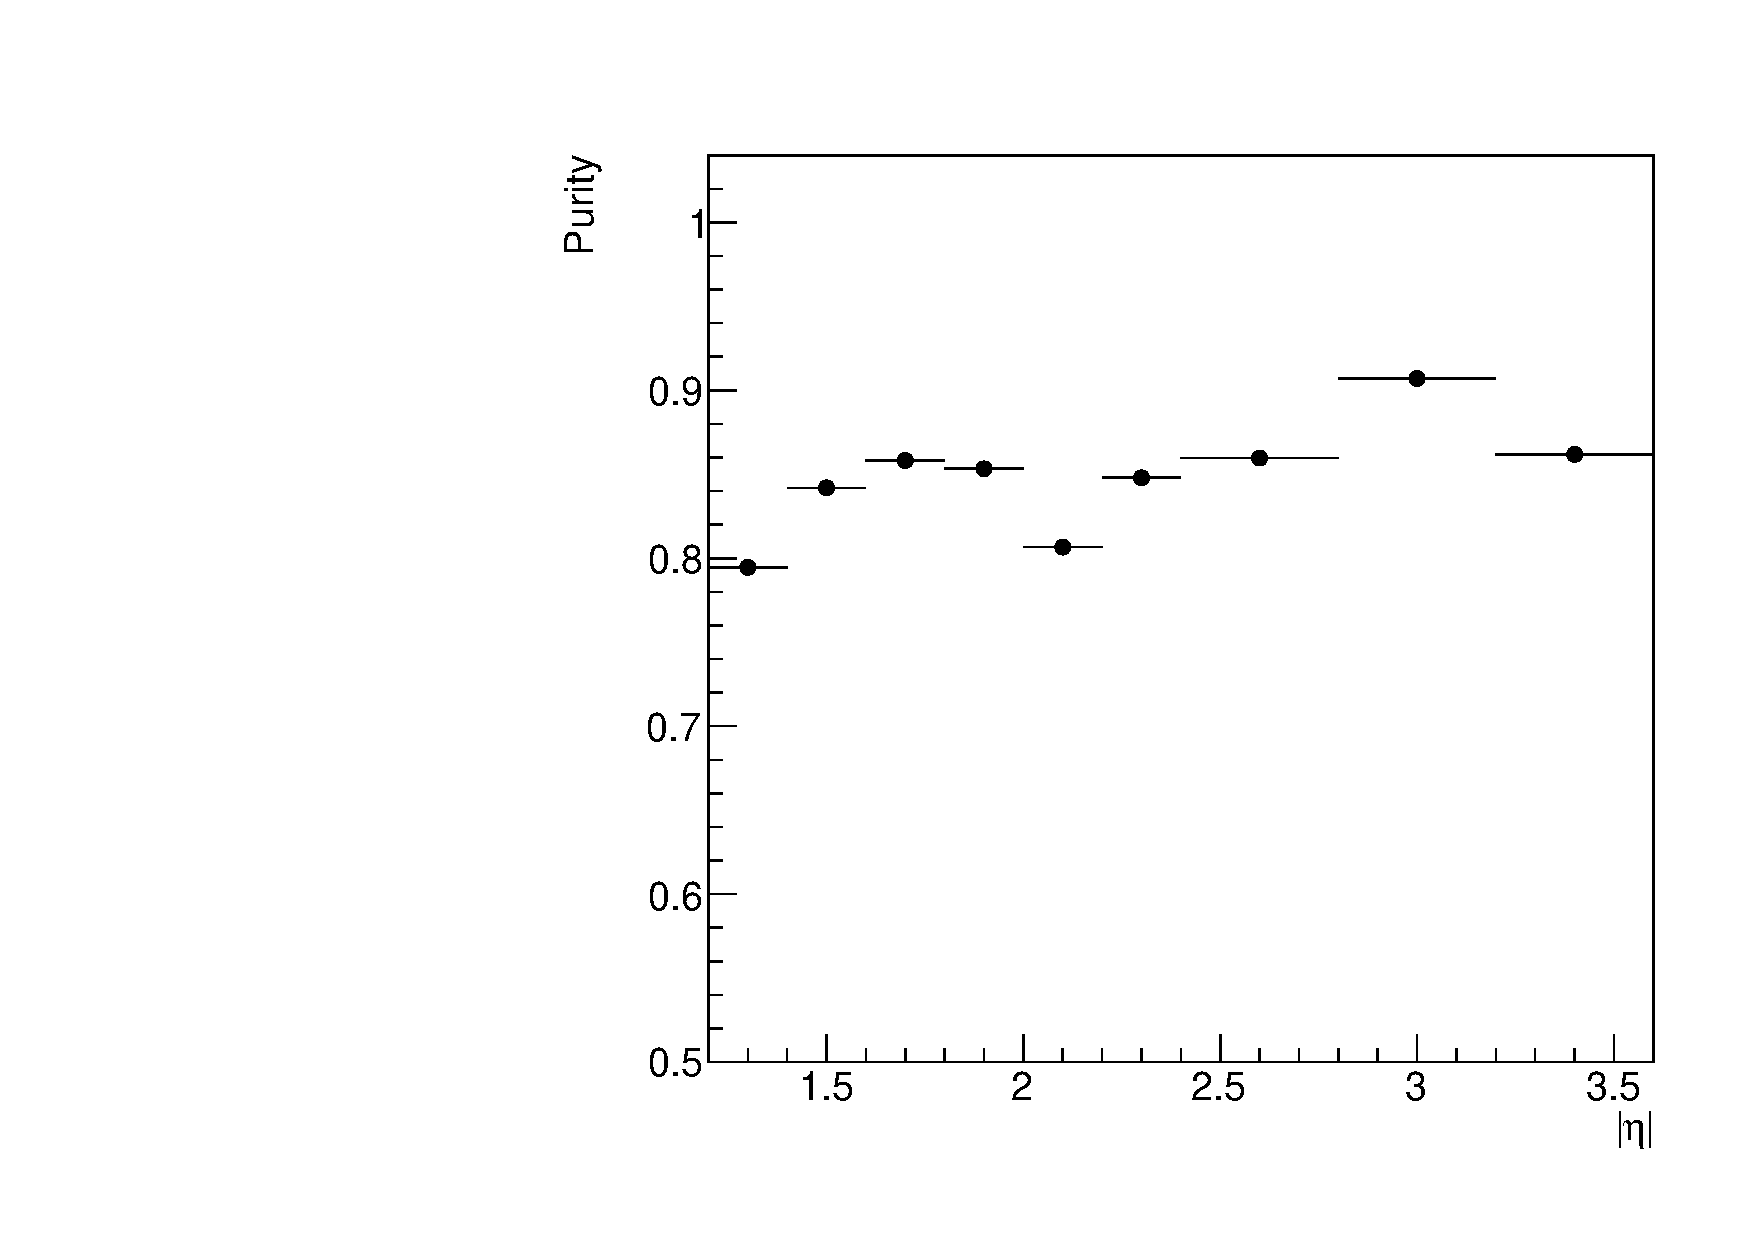
\includegraphics[width=0.45\textwidth]{figures/ZCF_purity_peak}%
  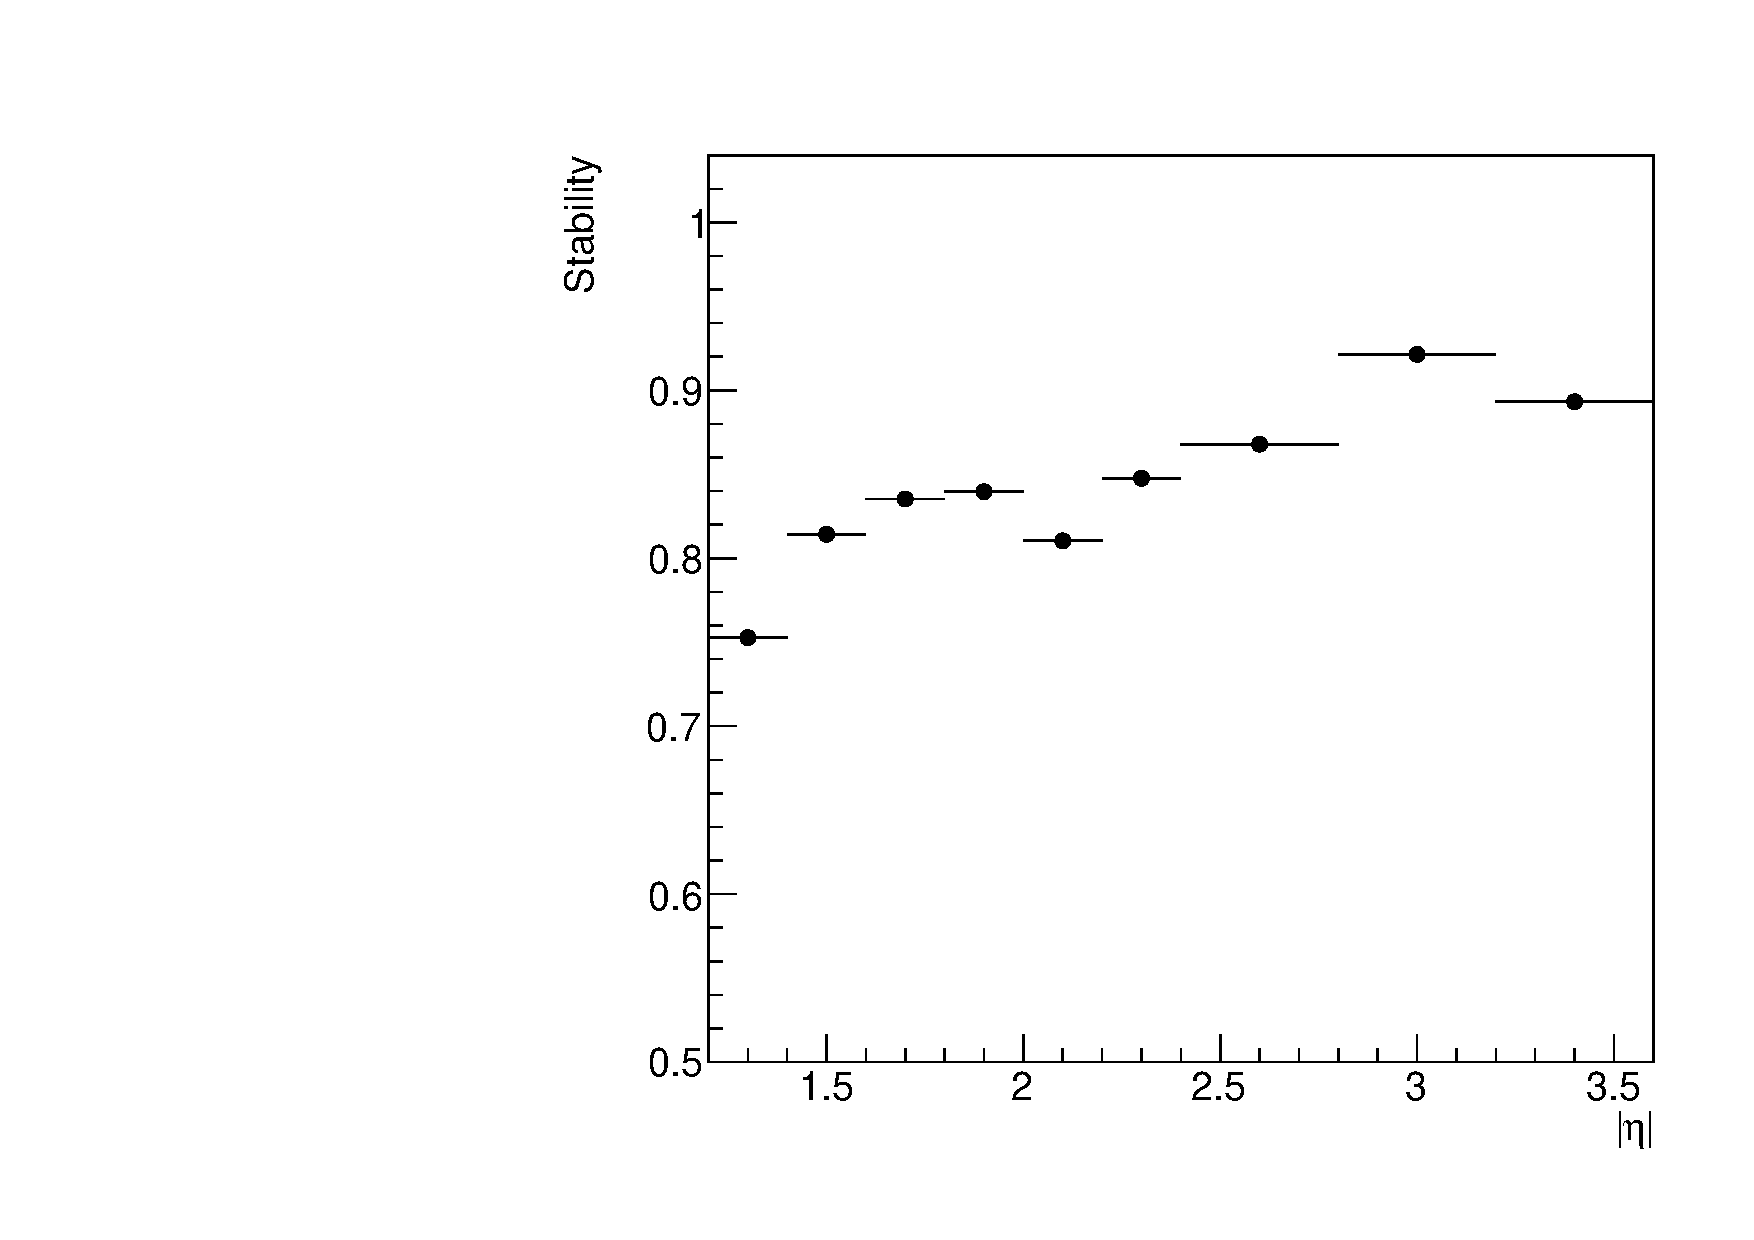
\includegraphics[width=0.45\textwidth]{figures/ZCF_stability_peak} \\
  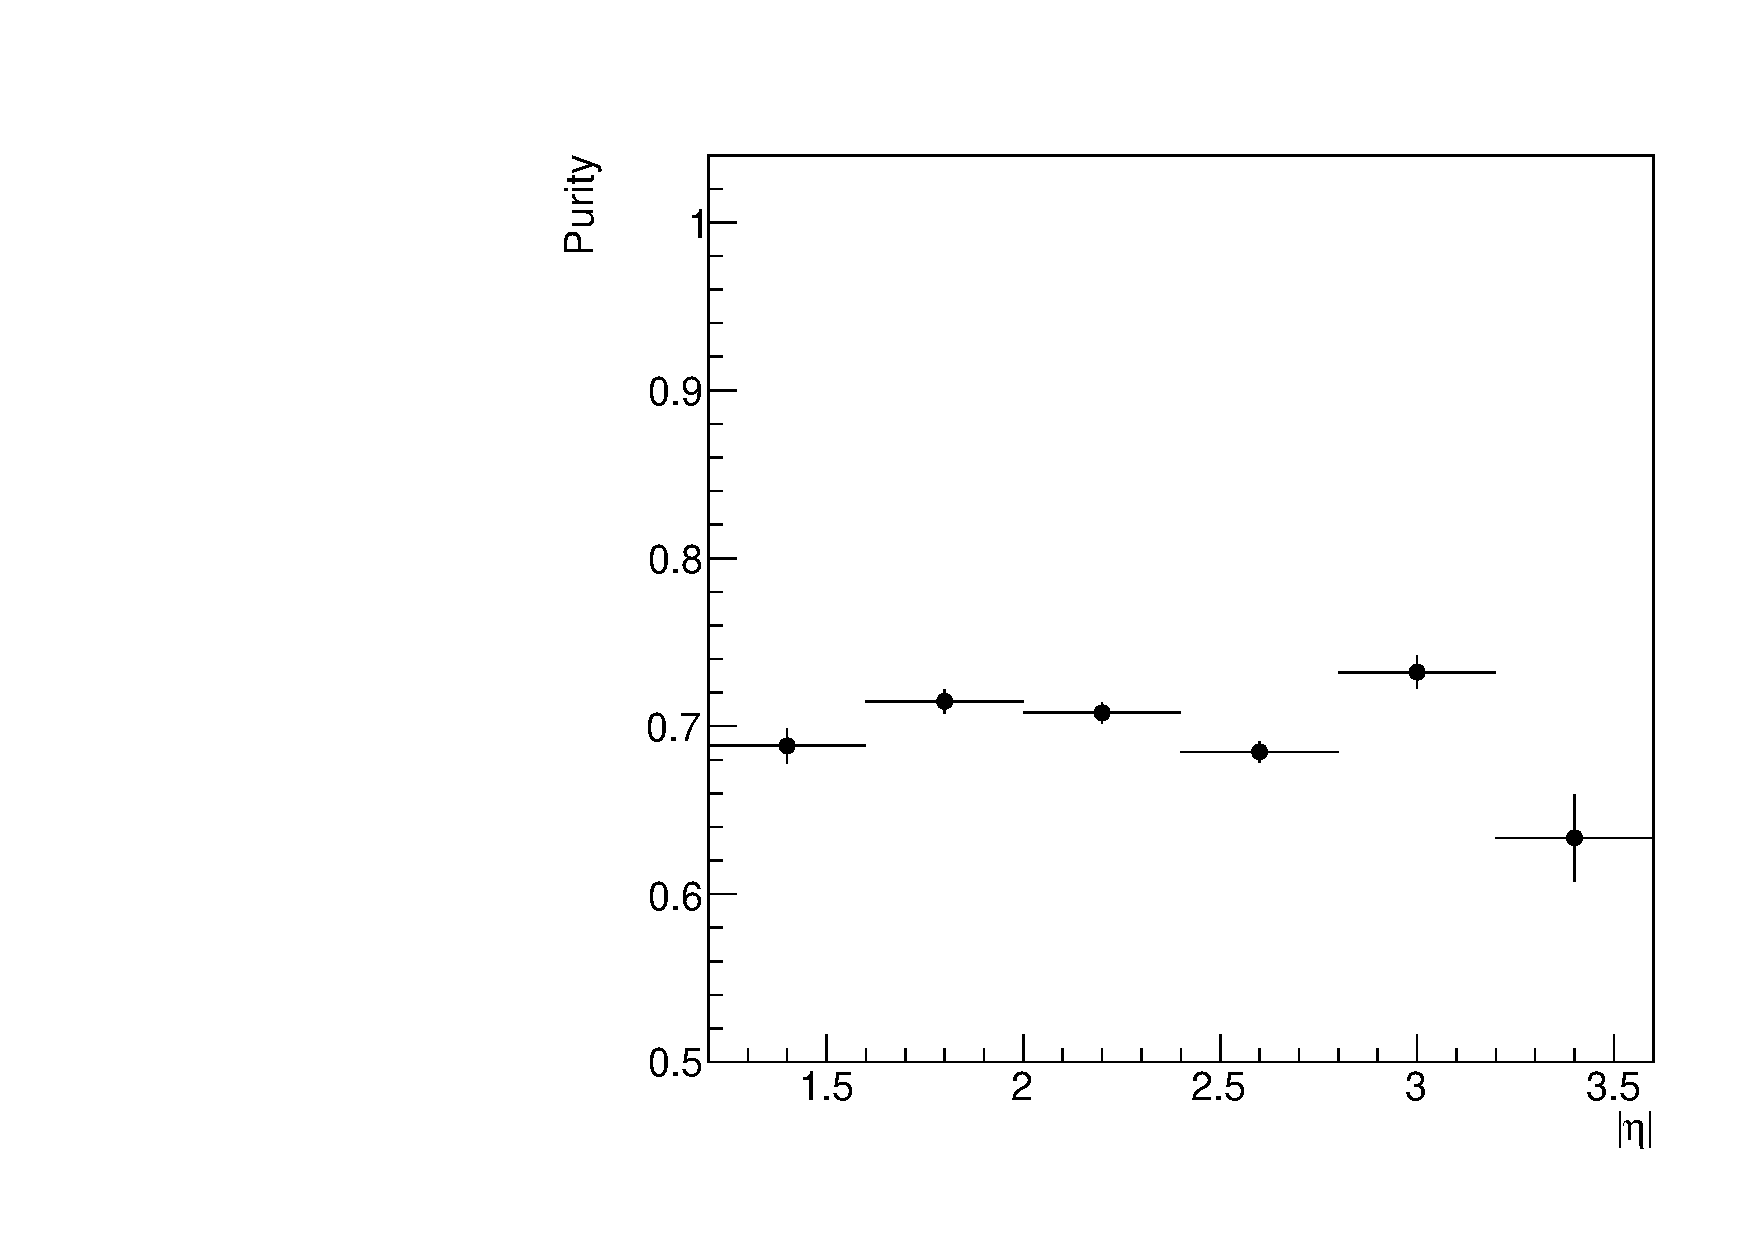
\includegraphics[width=0.45\textwidth]{figures/ZCF_purity_high}%
  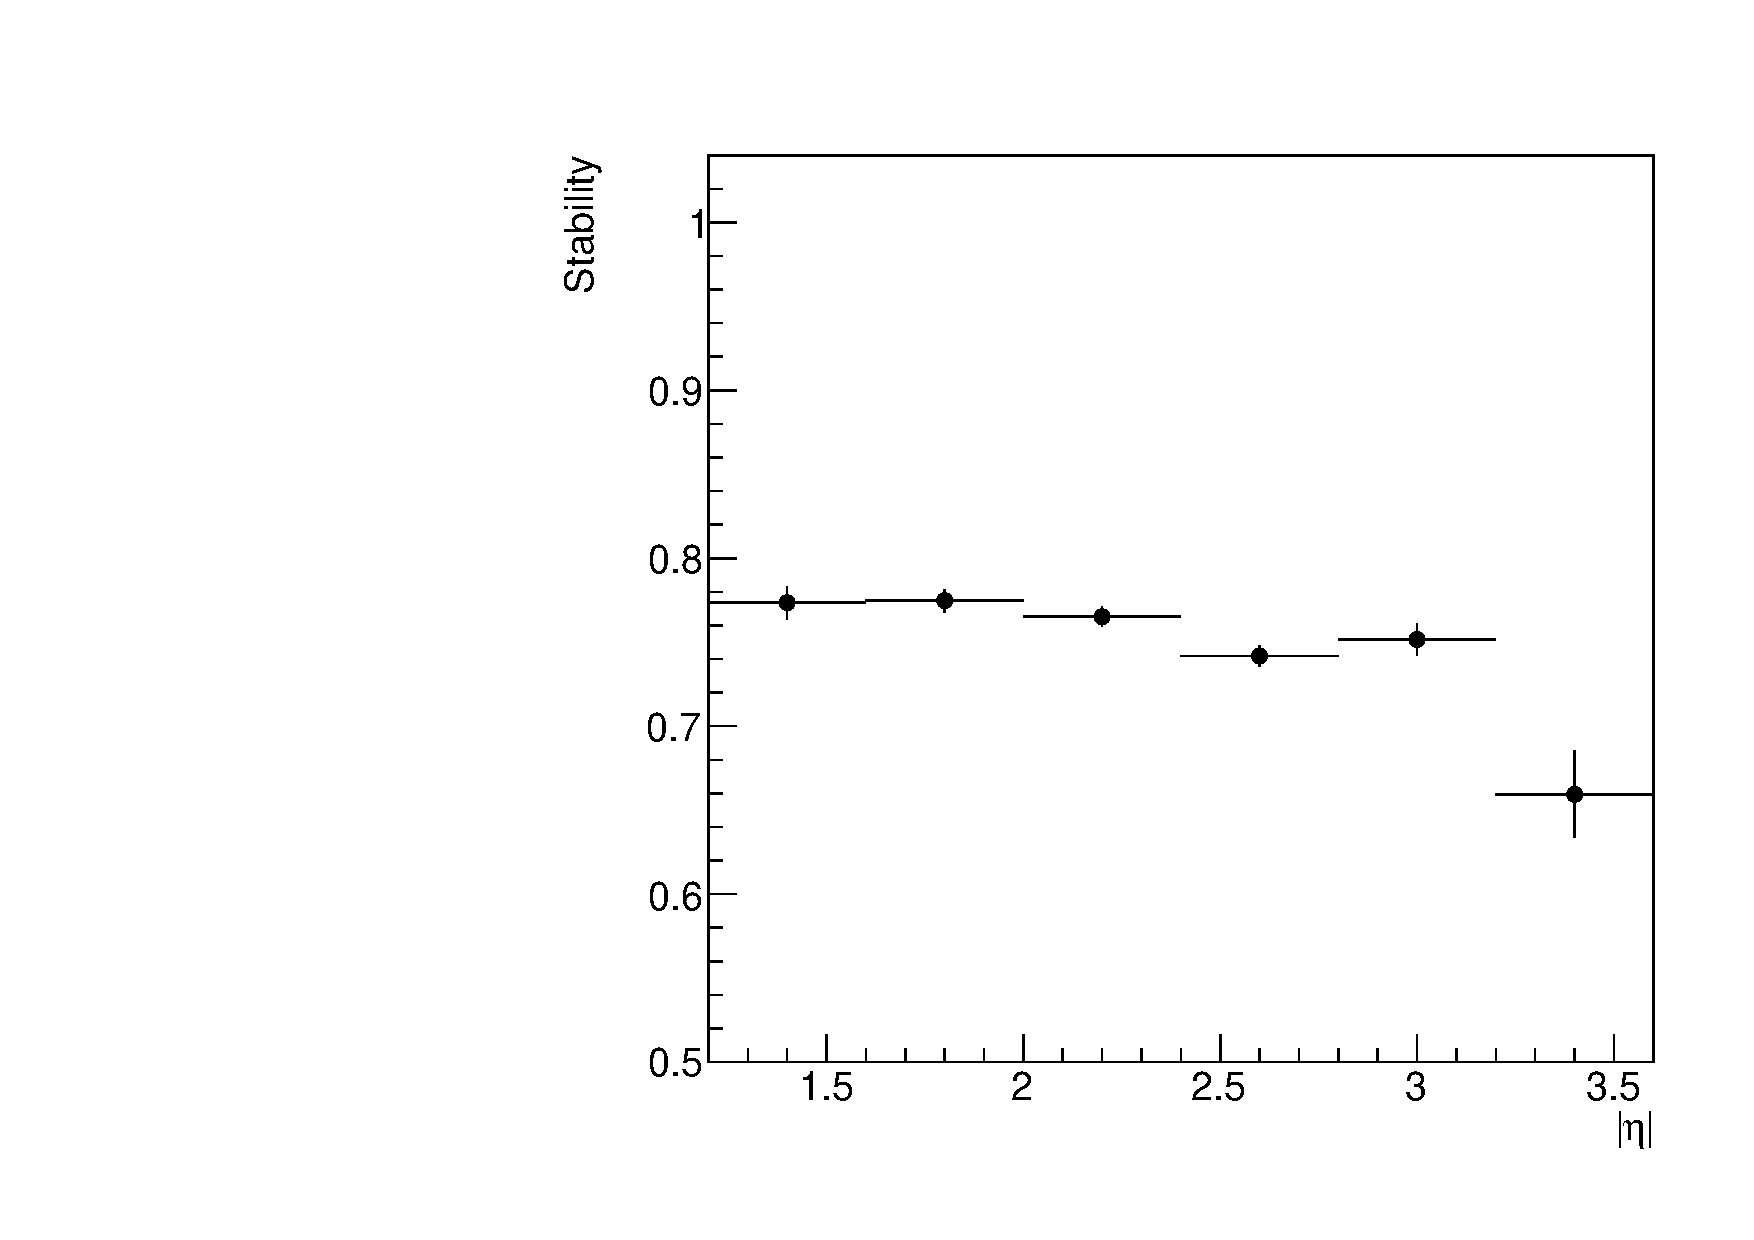
\includegraphics[width=0.45\textwidth]{figures/ZCF_stability_high} \\
  \caption{Purity (left) and stability (right) for the Z central-forward peak mass (top) and high mass (bottom) analyses.}
  \label{fig:ZeeCS_purity_stability}
\end{figure}

While calculating the $C$, $E$ and $A$ correction factors, there is a very important thing that must be taken into account, which is the QED final state radiation (FSR). The results of the MC generation are so-called {\itshape born level} leptons, which are the leptons before FSR. To simulate FSR there are two tools in use in the MC production chain: \Photos\, which is the main tool that is used, and \Sherpa\ which uses different FSR algorithm and is used for systematic uncertainties calculation. After the FSR simulation, the resulting final state leptons are called {\itshape bare leptons}. The bare leptons represent the result of the actual collision much closer than the born leptons, but because of the work of the clustering algorithms during reconstruction, bare leptons are impossible to reconstruct. To overcome this problem, the third level of FSR was introduced, which is {\itshape dressed leptons}. The dressed leptons are bare leptons with the inclusion of all FSR photons within the $\Delta R < 0.1$. The dressed leptons are the leptons that most closely represent the particles that are actually reconstructed by the reconstruction algorithms.

The calculation of the correction factors is always done on the born level, because the simulation on the born level is the best from the theoretical point of view (the FSR simulation is very approximate). The $C$, $E$ and $A$ then look like this:
\begin{equation}
C = \frac{N_\mathrm{MC, rec}}{N_\mathrm{MC, genBorn, cutexp}}\,, \;
E = \frac{N_\mathrm{MC, genBorn, cutexp}}{N_\mathrm{MC, genBorn, cutfid}}\,, \;
A = \frac{N_\mathrm{MC, genBorn, cutfid}}{N_\mathrm{MC, genBorn, all}}\,.
\end{equation}
And for the bare and dressed levels the cross-sections are calculated with good approximation by using the $\delta^\mathrm{bare}$ and $\delta^\mathrm{dressed}$ which are defined as:
\begin{equation}
\begin{split}
  \delta^\mathrm{bare} = \frac{N_\mathrm{MC, genBare, fidcut}}{N_\mathrm{MC, genBorn, fidcut}}\:\:\:&\mbox{and}\:\:\:
  \delta^\mathrm{dressed} = \frac{N_\mathrm{MC, genDressed, fidcut}}{N_\mathrm{MC, genBorn, fidcut}}\\
  \sigma_{fid}^\mathrm{Born} \cdot \delta^\mathrm{bare} =
  \sigma_{fid}^\mathrm{bare} \:\:\:\:\:\:&\mbox{and}\:\:\:\:\:\:
  \sigma_{fid}^\mathrm{Born} \cdot \delta^\mathrm{dressed} =
  \sigma_{fid}^\mathrm{dressed} \,.
\end{split}
\end{equation}

When it comes to Bayesian unfolding, all the coefficients mentioned above gets hidden inside the unfolding matrixes and are not observed directly. Yet we can see, that since the $A$ extrapolation coefficient deals with total cross-section, which we are not interested in, and that the $E$ coefficient is purely theoretical, and doesn't depend on experiment in any way, only on the set of the fiducial cuts that we apply. The only coefficient that can be regarded as a result of an experiment is thus the $C$ coefficient, which roughly represents the fraction of the total number of the $Z$ bosons produced, that got included in the analysis. For the 2011 \Zee\ CF analysis it was $\sim$42\% (see Sec.~\ref{sec:Results} for more details).

The differential cross-section measurement was done in absolute rapidity binning, which allows the later combination of the CC and CF analysis results. The binning is shown in Tabs.~\ref{tab:ZeeCS_bins_peak} and~\ref{tab:ZeeCS_bins_high}. The mass binning for the double-differential CF analysis had only two bins: the peak-mass window $66 < m_{ee} < 116$~GeV and the high-mass window $116 < m_{ee} < 150$~GeV.

\begin{table}
\centering
\begin{tabular}{c}
\hline\hline
Boundaries\\\hline
$1.20 < |y_{Z}| <1.40$\\
$1.40 < |y_{Z}| <1.60$\\
$1.60 < |y_{Z}| <1.80$\\
$1.80 < |y_{Z}| <2.00$\\
$2.00 < |y_{Z}| <2.20$\\
$2.20 < |y_{Z}| <2.40$\\
$2.40 < |y_{Z}| <2.80$\\
$2.80 < |y_{Z}| <3.20$\\
$3.20 < |y_{Z}| <3.60$\\
\hline\hline
\end{tabular}
\caption{Bins in $|y_{Z}|$ which are used for the \Zee\ CF analysis for peak mass window ($66 < m_{ee} < 116$~GeV).}
\label{tab:ZeeCS_bins_peak}
\end{table}

\begin{table}
\centering
\begin{tabular}{c}
\hline\hline
Boundaries\\\hline
$1.20 < |y_{Z}| <1.60$\\
$1.60 < |y_{Z}| <2.00$\\
$2.00 < |y_{Z}| <2.40$\\
$2.40 < |y_{Z}| <2.80$\\
$2.80 < |y_{Z}| <3.20$\\
$3.20 < |y_{Z}| <3.60$\\
\hline\hline
\end{tabular}
\caption{Bins in $|y_{Z}|$ which are used for the \Zee\ CF analysis for high mass window ($116 < m_{ee} < 150$~GeV).}
\label{tab:ZeeCS_bins_high}
\end{table}
